\documentclass{article}
\usepackage{graphicx}
\usepackage{float}

\begin{document}

\section*{Image Collection}
\IfFileExists{results/heaps/heaps.pdf}{
	\begin{figure}[H]
	\centering
	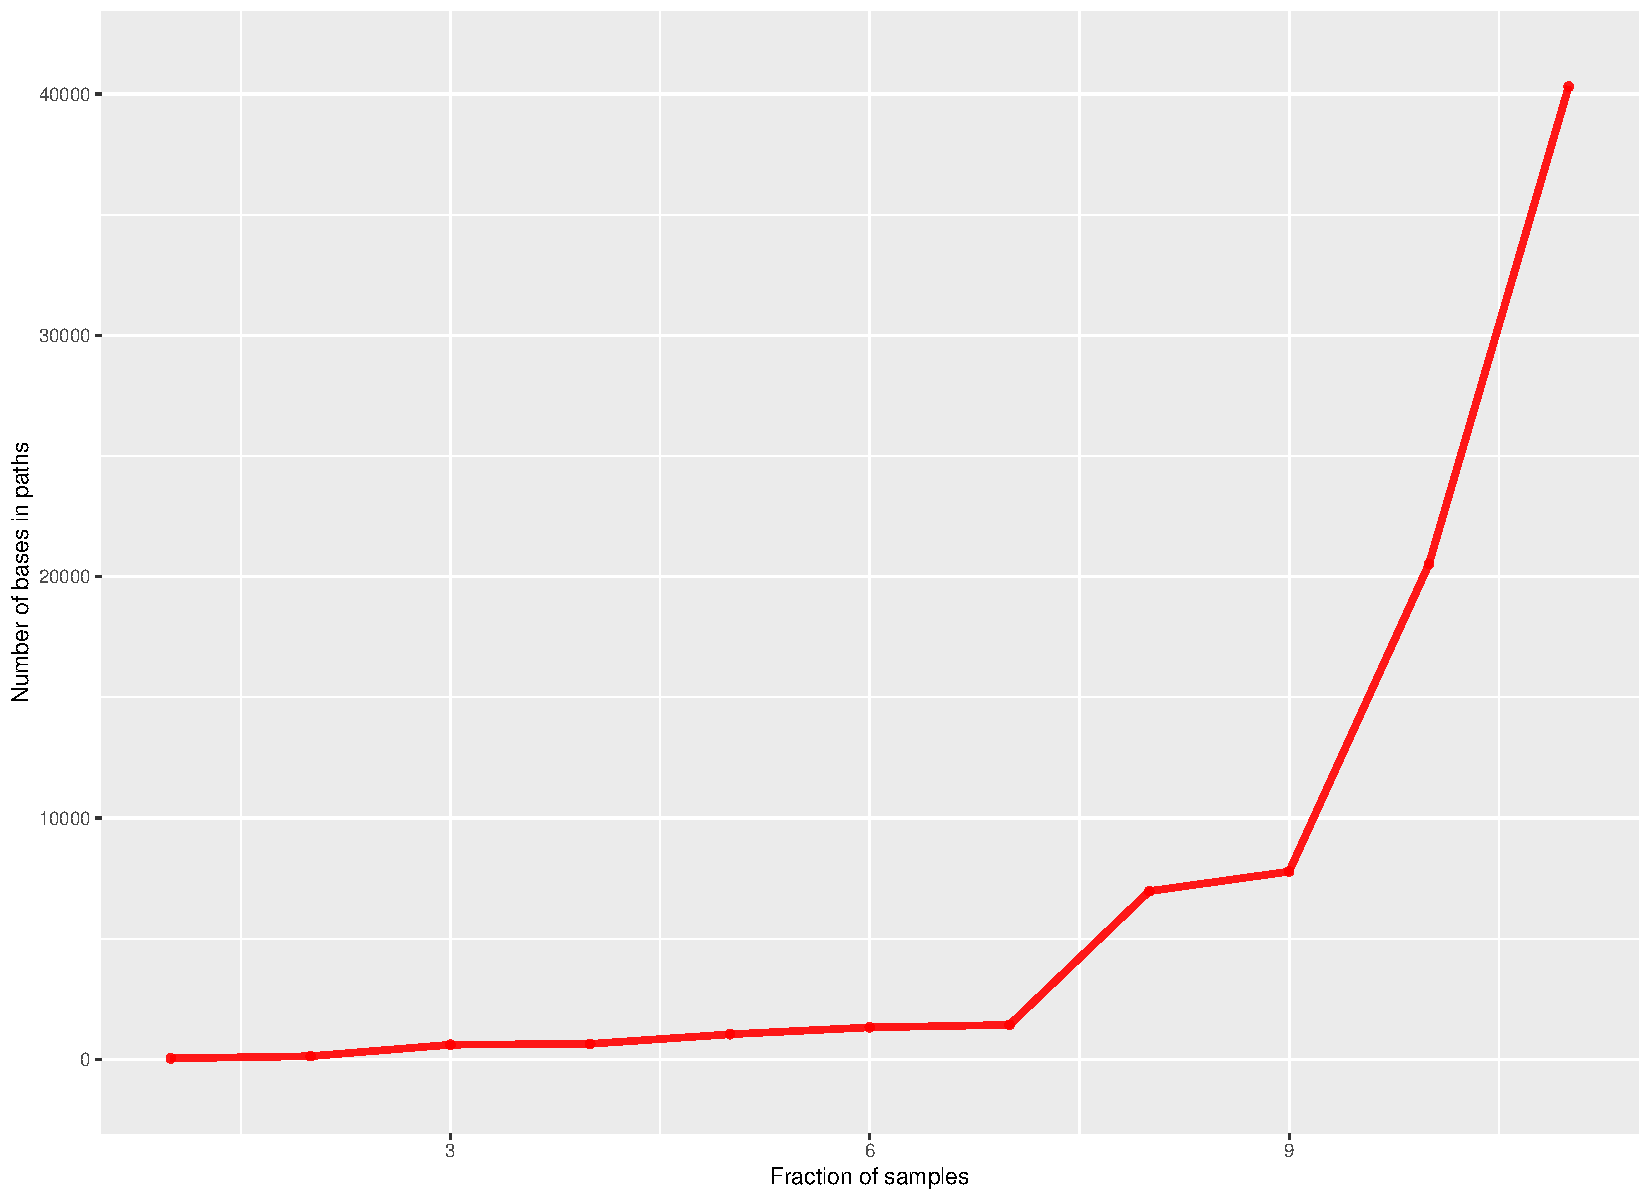
\includegraphics[width=0.8\textwidth]{results/heaps/heaps.pdf}
	\caption{Heaps output}
	\end{figure}
}{}

\IfFileExists{results/panacus/histgrowth.node.pdf}{%
    \begin{figure}[H]
        \centering
        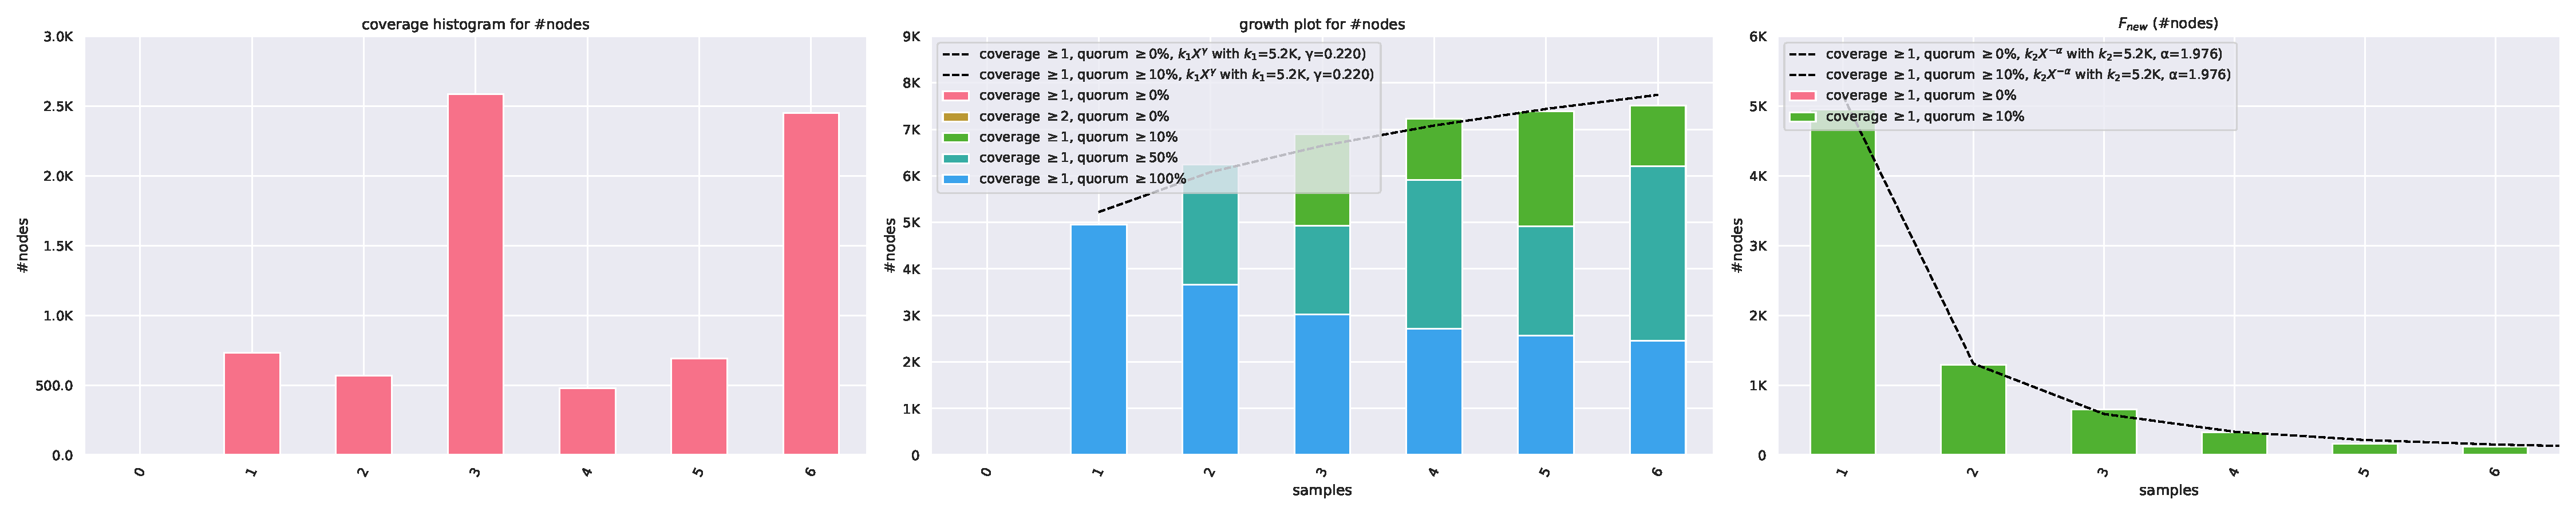
\includegraphics[width=0.8\textwidth]{results/panacus/histgrowth.node.pdf}
        \caption{Panacus output}
    \end{figure}
}{}

\IfFileExists{results/tree/tree.png}{%
    \begin{figure}[H]
        \centering
        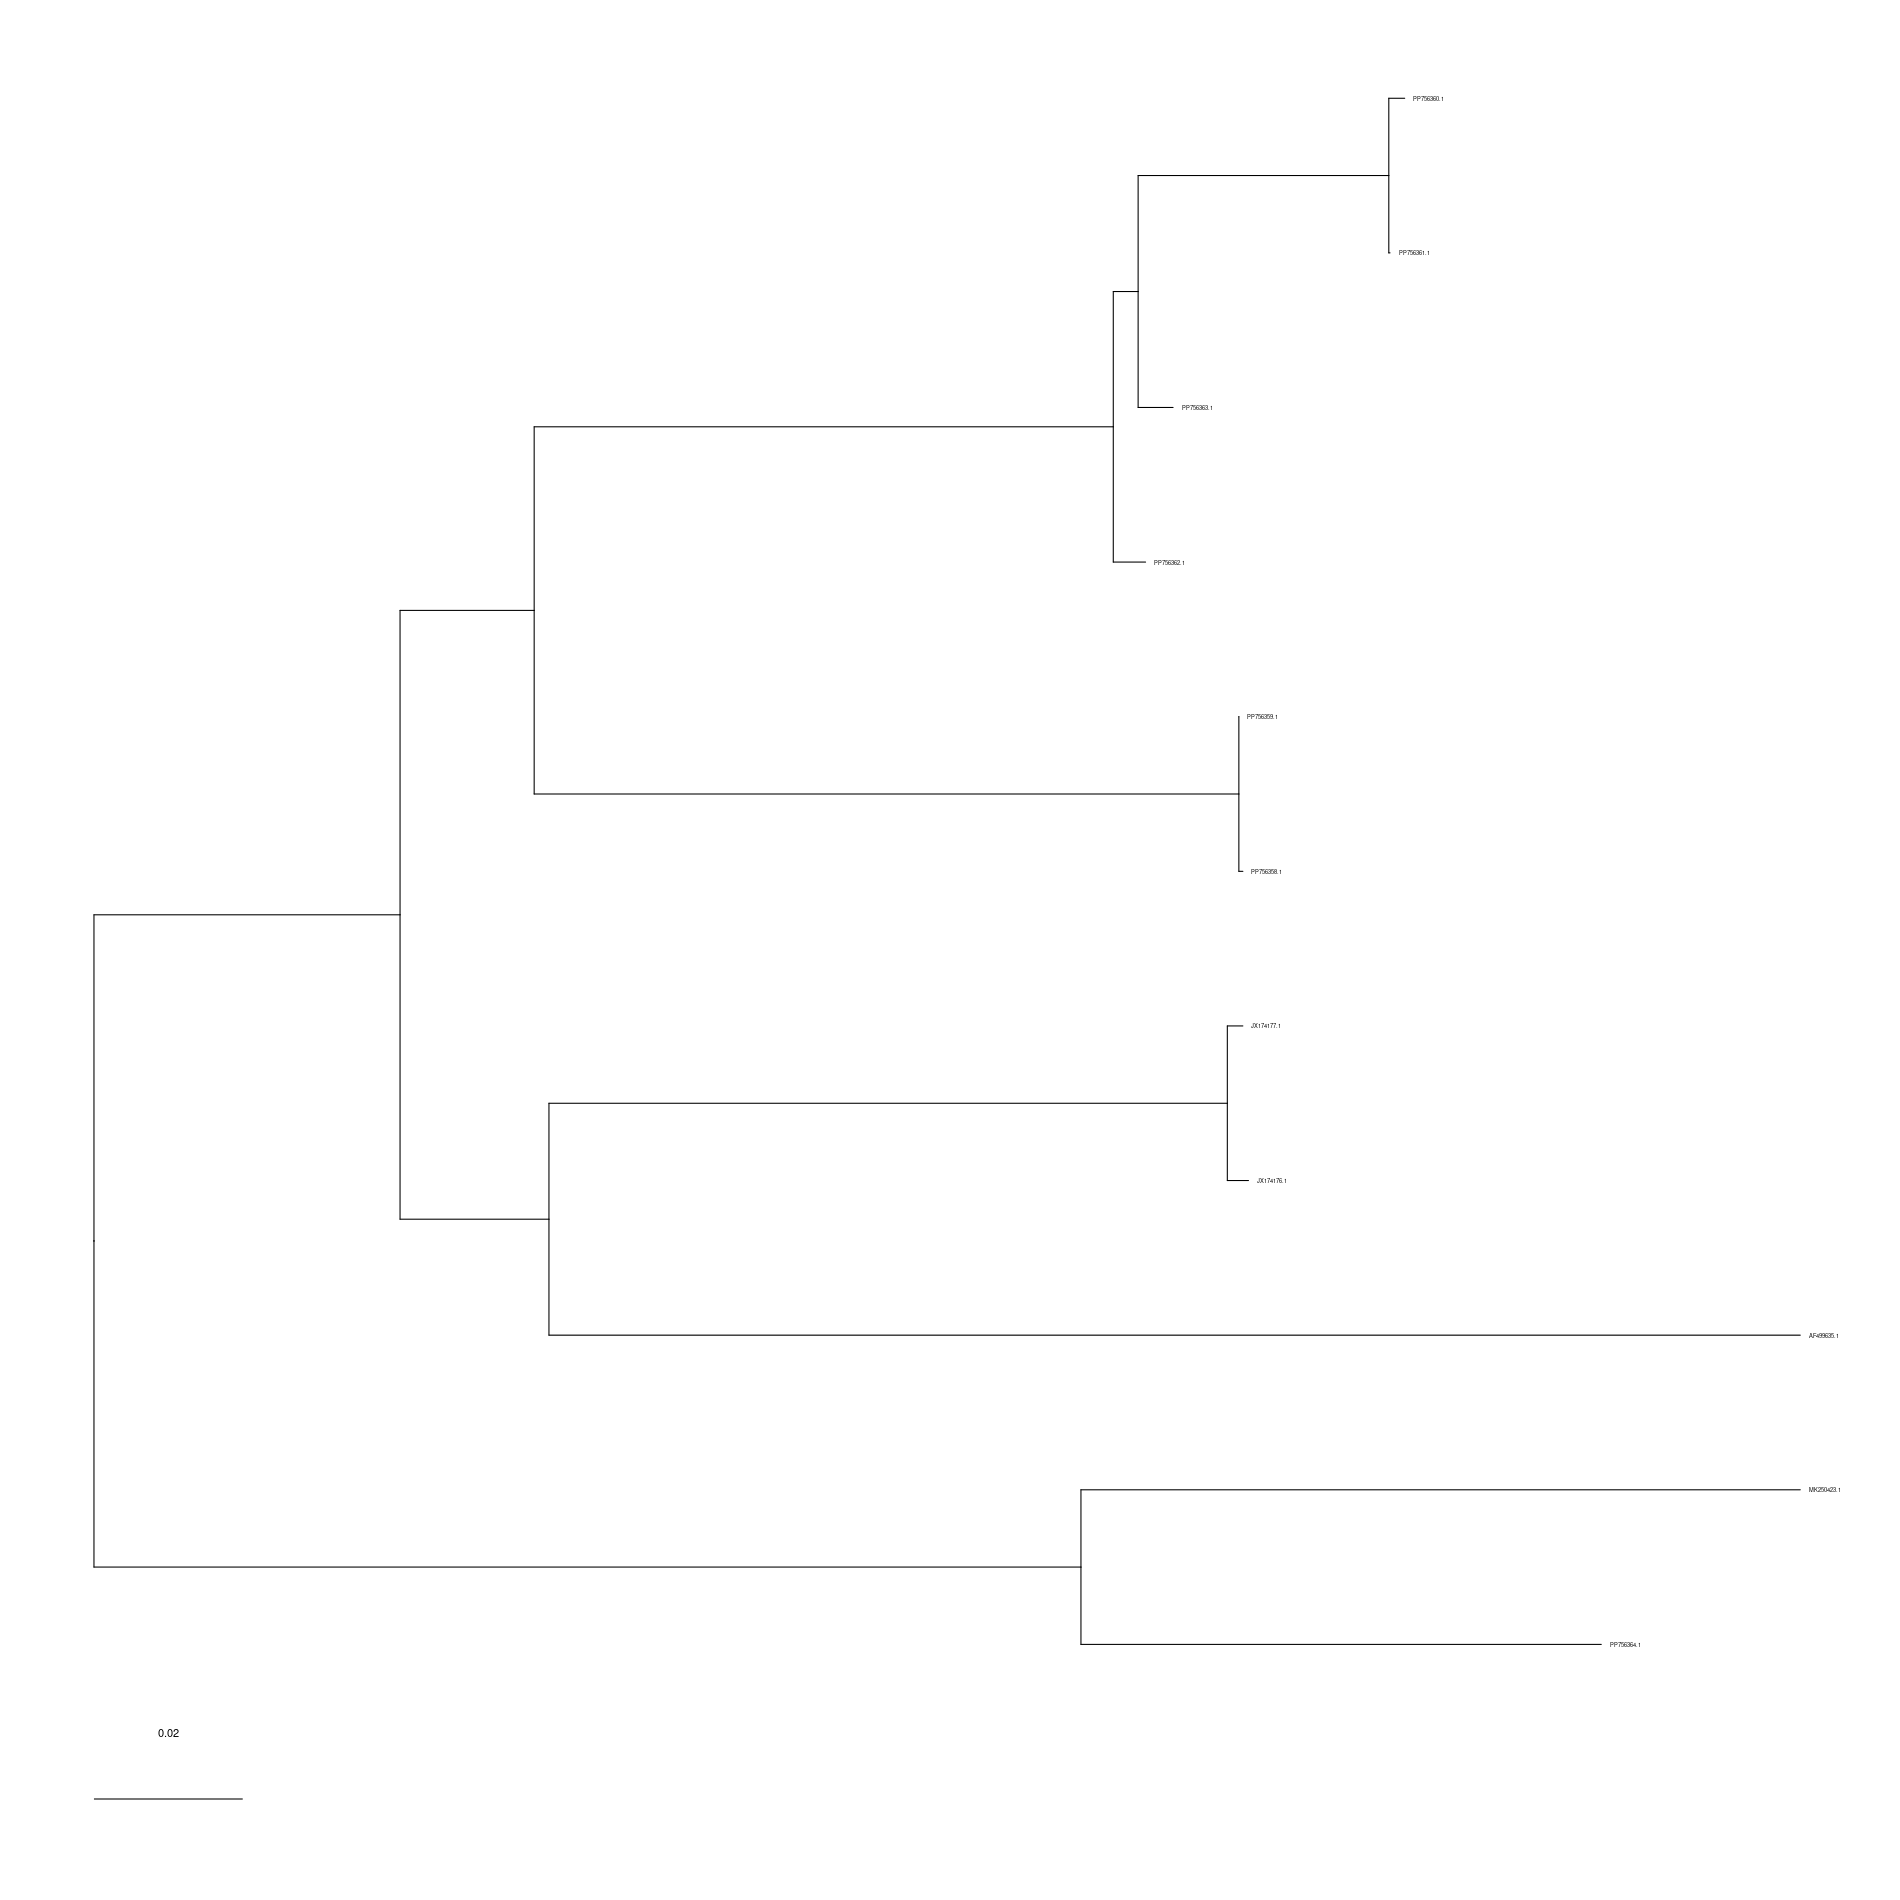
\includegraphics[width=0.8\textwidth]{results/tree/tree.png}
        \caption{Tree}
    \end{figure}
}{}

\IfFileExists{results/vg/out.vg.png}{%
    \begin{figure}[H]
        \centering
        
\includegraphics[width=0.8\textwidth]{results/vg/out.vg.png}
        \caption{Vg}
    \end{figure}
}{}

\IfFileExists{results/viz2/out.viz.png}{%
    \begin{figure}[H]
        \centering
        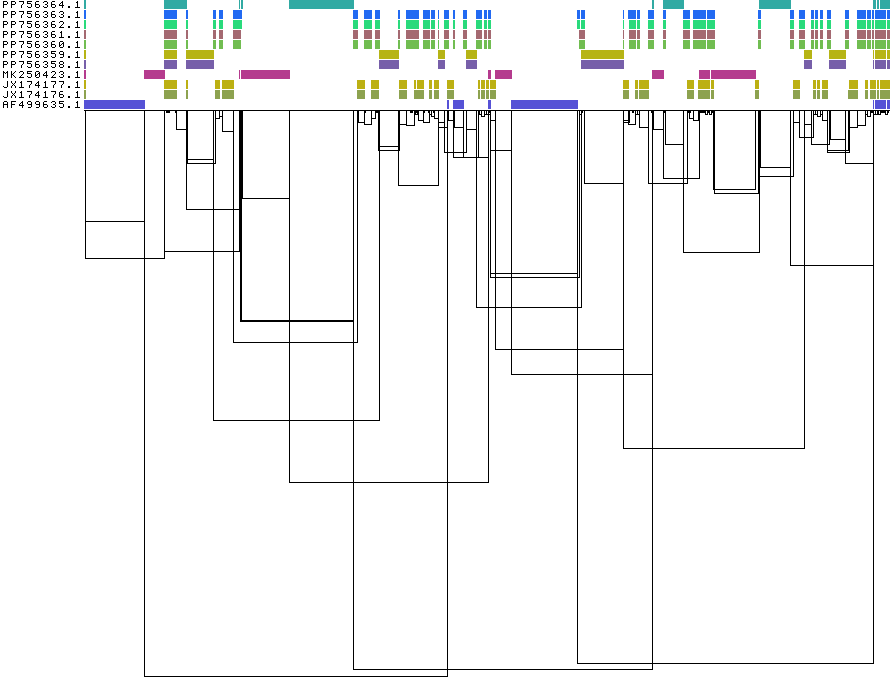
\includegraphics[width=0.8\textwidth]{results/viz2/out.viz.png}
        \caption{viz2}
    \end{figure}
}{}

\IfFileExists{results/pangrowth/pangrowth.pdf}{%
    \begin{figure}[H]
        \centering
        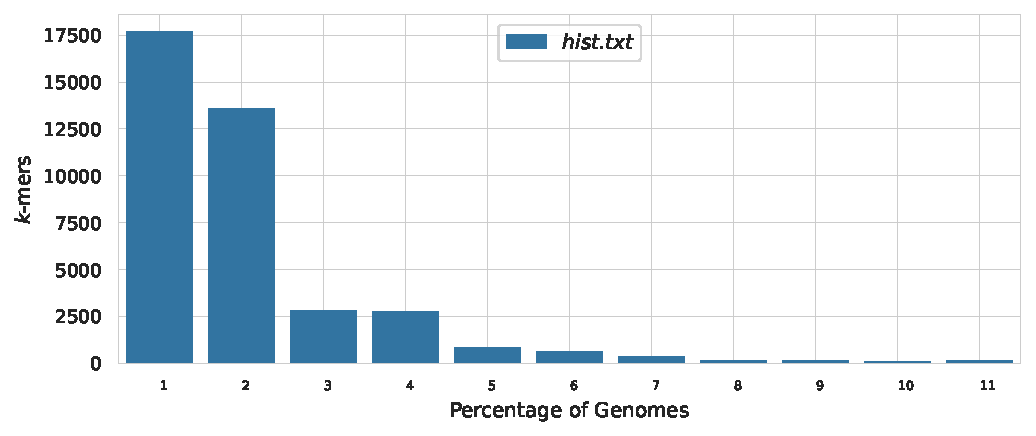
\includegraphics[width=0.8\textwidth]{results/pangrowth/pangrowth.pdf}
        \caption{Pangrowth Growth}
    \end{figure}
}{}

\IfFileExists{results/pangrowth/p_core.pdf}{%
    \begin{figure}[H]
        \centering
        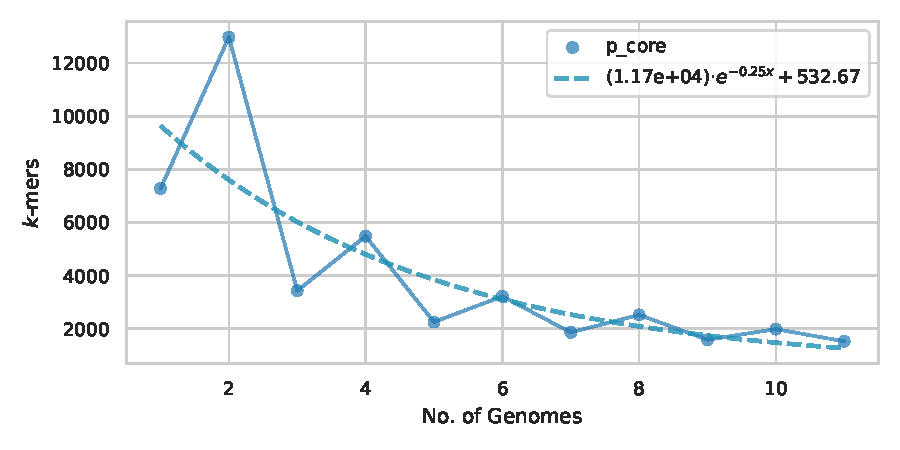
\includegraphics[width=0.8\textwidth]{results/pangrowth/p_core.pdf}
        \caption{Pangrowth Core}
    \end{figure}
}{}

\IfFileExists{results/newimage1.pdf}{%
    \begin{figure}[H]
        \centering
        \includegraphics[width=0.8\textwidth]{results/newimage1.pdf}
        \caption{New Image 1}
    \end{figure}
}{}

\IfFileExists{results/newimage2.png}{%
    \begin{figure}[H]
        \centering
        \includegraphics[width=0.8\textwidth]{results/newimage2.png}
        \caption{New Image 2}
    \end{figure}
}{}

\end{document}

